\documentclass[11.5pt]{sig-alternate} % sets document style to sig-alternate
% packages
% typesetting
%\usepackage{dirtytalk} % typset quotations easier (\say{stuff})
\usepackage{hanging} % hanging paragraphs
\usepackage[defaultlines=3,all]{nowidow} % avoid widows
\usepackage[pdfpagelabels=false]{hyperref} % produce hypertext links, includes backref and nameref
\usepackage{xurl} % defines url linebreaks, loads url package
\usepackage{microtype}
%\usepackage[super]{nth} % easily create superscript ordinal numbers with \nth{x}\
\usepackage{enumitem}
% layout
\usepackage{enumitem} % control layout of itemize, enumerate, description
\usepackage{fancyhdr} % control page headers and footers
\usepackage{float} % improved interface for floating objects
%\usepackage{multicol} % intermix single and multiple column pages
% language
\usepackage[utf8]{inputenc} % accept different input encodings
\usepackage[english]{babel} % multilanguage support
% misc
\usepackage{graphicx} % builds upon graphics package, \includegraphics
%\usepackage{lastpage} % reference number of pages
%\usepackage{comment} % exclude portions of text (?)
\usepackage{xcolor} % color extensions
\usepackage[backend=biber, style=apa]{biblatex} % sophisticated bibliographies % necessary for HTML to display author info and date on abstract page
\usepackage{csquotes} % advanced quotations, makes biblatex happy
\usepackage{authblk} % support for footnote style author/affiliation
% tables and figures
\usepackage{tabularray}
%\usepackage{array} % extend array and tabular environments
\usepackage{caption} % customize captions in figures and tables (rotating captions, sideways captions, etc)
%\usepackage{cuted} % allow mixing of \onecolumn and \twocolumn on same page
\usepackage{multirow} % create tabular cells spanning multiple rows
%\usepackage{subfigure} % deprecated, support for manipulation of small figures
%\usepackage{tabularx} % extension of tabular with column designator "x", creates paragraph-like column whose width automatically expands
%\usepackage{wrapfig} % allows figures or tables to have text wrapped around them
%\usepackage{booktabs} % better rules
% dummy text
%\usepackage{blindtext} % blind text dummy text
%\usepackage{kantlipsum} % Kant style dummy text
\usepackage{lipsum} %lorem ipsum dummy text
% other helpful packages may be booktabs, longtable, longtabu, microtype

\pagestyle{fancy} % sets pagestyle to fancy for fancy headers and footers

% header and footer
% modern way to set header image
\renewcommand{\headrulewidth}{0pt} % defines thickness of line under header
\renewcommand{\footrulewidth}{0pt} % defines thickness of line above header
\setlength\headheight{80.0pt} % sets height between top margin and header image, effectively moves page contents down
\addtolength{\textheight}{-80.0pt} % seems to affect the lower height. maybe only works properly if footer numbers enabled?
\fancyhf{}
\fancyhead[CE, CO]{
\includegraphics[width=\textwidth]{headerImage.png}}
% footer
%\fancyfoot[LE,LO]{Article Title Here \\ DOI: }% left footer article title and doi
%\fancyfoot[CE,CO]{{}} % center footer empty
%\fancyfoot[RE,RO]{\thepage} % right footer page numbers
%\pagenumbering{arabic} % arabic (1, 2, 3) numbering in footer

\hypersetup{colorlinks=true,urlcolor=blue} % sets link color to blue
\urlstyle{same} % sets url typeface to same as rest of text

% set caption and figure to italics, label bold, left align captions, does not transfer to HTML
\DeclareCaptionFormat{custom}
{
    \textbf{\textit{\large #1#2}}\textit{\large #3} % #1 is the "Table 1" or "Figure 1" part, #2 is the separator (":"), #3 is the caption
}
\captionsetup{format=custom}
\captionsetup{justification = raggedright, singlelinecheck = false}

%this next bit is confusing, but essentially changes the width of the abstract. Seems to have been copied from this https://tex.stackexchange.com/questions/151583/how-to-adjust-the-width-of-abstract
\let\oldabstract\abstract
\let\oldendabstract\endabstract
\makeatletter %changes @ catcode to enable modification (in parsep)
\renewenvironment{abstract} %alters the abstract environment
{\renewenvironment{quotation}%
               {\list{}{\addtolength{\leftmargin}{1em} % change this value to add or remove length to the the default ?
                        \listparindent 1.5em%
                        \itemindent    \listparindent%
                        \rightmargin   \leftmargin%
                        \parsep        \z@ \@plus\p@}%
                \item\relax}%
               {\endlist}%
\oldabstract}
{\oldendabstract}
\makeatother %changes @ catcode to disable modification

\begin{document}

\title{Exploring User Interface Improvements for Software Developers who are Blind}

\author[1]{\large \color{blue}Guarionex Salivia}
\author[1]{\large \color{blue}Flint Million}
\author[1]{\large \color{blue}Megan Bening}

\affil[1]{Minnesota State University-Mankato}

\toappear{}
%% ABSTRACT
\maketitle
\begin{@twocolumnfalse} 
\begin{abstract}
\item 
\textit {Software developers who are blind and interact with the computer non-visually face unique challenges with information retrieval. We explore the use of speech and Braille combined with software to provide an improved interface to aid with challenges associated with information retrieval. We motivate our design on common tasks performed by students in a software development course using a Microprocessor without Interlocked Pipeline Stages (MIPS) architecture simulation tool. We test our interface via a single-subject longitudinal study, and we measure and show improvement in both the user’s performance and the user experience.}
\\ \\
Keywords: Accessibility; Blindness; Visual Impairments; Braille; Screen reader technology; Software development
\end{abstract}
\end{@twocolumnfalse}

%% AUTHOR INFORMATION

\textbf{*Corresponding Author, Guarionex Salivia}\\
\href{mailto:  salivia@mnsu.edu}{(salivia@mnsu.edu)} \\
\textit{Submitted  October, 2019}\\
\textit{Accepted February 4, 202} \\
\textit{Published online July 23, 2020} \\
\textit{DOI:10.14448/jsesd.12.0011} \\
\pagebreak
\clearpage

\begin{large}
\section*{INTRODUCTION}

People who are blind face unique challenges as software developers. Screen reading technology is often unable to adequately represent the complex and dynamic nature of modern application interfaces often used for software development. Complex interfaces make the task of information seeking and retrieval particularly challenging to developers who are blind. Our main goal is to help individuals who are blind with the problem of information retrieval in a non-visual manner from a graphical user interface. We are particularly interested with graphical user interfaces related to software development such as text editors and integrated development environments (IDEs). Information retrieval has been shown to be a prevalent problem amongst individuals who are blind interacting with technology, especially software developers (Mealin \& Murphy-Hill, 2012). There are an estimated 19 million software developers worldwide, with an expected increase to at least 25 million by the year 2020 (Evans Data Corporation, 2014). Out of the plethora of software developers, we do not know exactly how many of them are blind or visually impaired. However, according to a survey conducted by Stack Overflow, a prominent software development resource website, more than 600 respondents identified as blind (Stack Overflow, 2017).

Modern software development tools are quite different from those used in years past. Today, IDEs provide highly dynamic, rich interfaces for developers. These interfaces facilitate productivity through their extensive visualization capabilities and organizational display of content. This augments the complexity of the information retrieval problem, because these interfaces provide information contextually via visual cues, which are clearly not specifically designed for individuals who are blind and may not work with existing accessibility tools such as screen readers. Therefore, those who are blind or visually impaired often find IDEs to be challenging to work with, and in many situations completely unusable even with the use of screen reading technology (Lazar, Allen, Kleinman, \& Malarkey, 2007).

In our work, we explore the use of Braille as a possible option to improve accessibility for software developers who are blind. One reason we concentrate on Braille as an option is based on reports by the American Printing House for the Blind. Out of their 27,212 student members currently enrolled in elementary through post-secondary education, 3,781 considered Braille to be their primary reading medium (American Printing House for the Blind, 2013). When we look at the intersection between software developers and users of Braille, we see that there is a big potential for Braille-based user interfaces to aid with information retrieval. Half of the participants in a study by Mealin and Murphy-Hill (2012) reported using a Braille display for software development. Furthermore, though Braille is introduced early in education, we have not seen recent work on developing more effective use of Braille when interacting with computers.

In this work, we develop a software add-on to an educational programming tool used in a university course to add functionality that provides a Braille user with enhanced ability to locate information and interact with the user interface. A developer is usually aware of the information they need to find. For developers who are not blind, IDEs provide information contextually via visual cues and layout allowing the developer to visually locate desired information while simultaneously ignoring less important content. On the other hand, users who are blind make use of proxies such as the cursor to navigate the information that is displayed. A contextual layout of information does not help a user who is blind because he or she would have to navigate away from the current position to find the relevant information, and then relocate to their previous focus manually. Our software allows the user to specify contextual information from the visual user interface (UI) that will be displayed in Braille regardless of where the user’s cursor is positioned, thus facilitating information retrieval. Additionally, the software assists the developer with parsing complex data structures represented in code that are very difficult to interpret with speech alone.

We perform a user experience study to measure the subjective and objective change in our student participant’s performance while interacting with an IDE which is part of a learning tool that utilizes the Microprocessor without Interlocked Pipeline Stages CPU architecture (MIPS). By assisting with information retrieval, we expect that our method will improve student developers’ abilities to complete tasks in a reasonable time and improve their experience while working in development environments.

\section*{RELATED WORK}

Historically, computer interfaces were largely character-based. When display devices were developed, the interface presented on screen was linear, textual, and command based. When computer interfaces were text-based, users who are blind found that they were able to access and use computers at roughly the same performance level as their sighted peers (Alexander, 1998). Speech synthesis technology provided auditory access to the computer’s output, and the linear nature of commands lent itself well to the linear nature of spoken word access.

As graphical user interfaces (GUIs) became more prevalent, people who are blind quickly found themselves less and less able to work with the computer with the same efficiency, speed and capability as their sighted peers (Lazar et al., 2007; Alexander, 1998). While screen-reading and Braille display access technology has continuously been adapted and improved, many such efforts at improving accessibility of GUIs require software developers to follow prescribed standards, often via specialized Application Programming Interfaces (APIs), to allow their software to be used effectively and efficiently by people who are blind. Initiatives such as Microsoft’s Active Accessibility were an early attempt to standardize access to graphical elements by users with disabilities (Lazar et al., 2007). However, no standard to implement such APIs was in place at the time. In fact, implementing accessibility required additional efforts on the part of the software publisher. Due to the time and effort required, these efforts were focused on mainstream application software and not on software development tools. In a CNN interview, Curtis Chong, former president of the National Federation of the Blind’s Science Division, reported his own personal struggles with the advancing GUI technology as a software developer (Alexander, 1998). He specifically stated that his performance decreased as a result of the graphical tool kit requiring you to drag and drop items on the screen.

The primary method of accessing GUIs for computer users who are blind is the screen reader. Screen readers have become extremely prevalent among users who are blind. A survey taken by WebAIM (Web Accessibility in Mind, a non-profit organization) found that 93\% of respondents reporting a significant visual impairment were regular users of screen reading technology (WebAIM, 2013).

Screen readers were designed to read and interpret common application interfaces. The GUIB (Textual and Graphical User Interfaces for Blind People) and Mercator projects are early efforts to provide accessibility of graphical user interfaces (GUIs) to visually impaired users (Mynatt \& Weber, 1994; Edwards, Mynatt, \& Stockton, 1994). Research efforts to provide non-visual GUI accessibility have shifted to web-based interfaces as web-application development became more prevalent. (Takagi, Saito, Fukuda, \& Asakawa, 2007; Lazar et al., 2007; K. \& C., 2014).

Screen readers extend the command set used to interact with the computer by adding commands which are specific to the needs of speech output. Such commands may include announcing the text on which the cursor is currently located, announcing the position of the cursor, and changing the rate or volume of the synthesized speech.

The use of Braille to enhance accessibility to computers for individuals who are blind has been explored since the 1970s. In 1971, the first Braille embossing device was released. Braille embossers allow a person to produce hard-copy Braille on paper from a computer. In 1982, Telesensory Inc. released the VersaBraille, the first electronic refreshable Braille terminal for computers available in the United States (Van Gerven \& Taylor, 2009), based on a patent received in 1975 by the founder of Handy Tech of Germany (Handy Tech, n.d.). Refreshable Braille displays are devices that display the transmitted text in an array of electronic Braille cells. These cells use mechanical actuators, often using piezoelectric technology, to allow them to instantly produce any Braille character, and just as quickly "refresh" themselves to display a different character. This allows the user to access computer information via tactile output, using the Braille written language. Additionally, many contemporary Braille displays can also function as input devices, allowing the user to input information into the computer using the Braille language.

Also, during the 1980s, Braille "notetaker" devices were introduced, providing the user with the ability to both input text using the Braille code as well as read content using both synthetic speech and refreshable Braille. A popular early device was known as the Braille n’Speak and was developed by Blazie Engineering. Notetakers used preinstalled custom software designed and written specifically for their use case. These devices allowed a Braille user to perform functions similar to a PDA device such as maintaining an address book and calendar and taking notes but did not provide access to mainstream computing interfaces on their own.

As screen reader software was developed and improved, the ability to represent content in Braille as well as via speech was developed. Popular screen readers such as Job Access With Speech (JAWS), Non-Visual Desktop Access (NVDA) and Apple’s VoiceOver have Braille output support. The simplest mode of operation is to simply display in Braille the same text which is being spoken aloud. However, because a Braille display is simply a row of independently addressable Braille cells, there exists significant potential to improve accessibility by directly interacting with the Braille cells in novel ways. Screen readers do take advantage of this for some use cases, such as "status cells" which allow a small number of cells to be designated such that they display various codes contextually relevant to the current operation (Freedom Scientific, 2014). For example, a status cell might indicate whether the user is currently focused on a check box, button, or text field.

Despite many years of innovation and further developments in screen reader technology, a software developer who is blind still faces unique challenges today. Access to information on a computer by a person who is blind is often linear (Edwards, Mynatt, \& Stockton, 1994; WebAIM, 2013). Using a screen reader, the individual will access information either audibly, as a stream of spoken words and/or sound effects, or through a Braille display device. Modern integrated development environments (IDEs) typically expose many types of contextually sensitive information at the same time on the screen. These developers may find it challenging, frustrating, or even impossible to keep up with the flood of information while seeking out relevant bits of content and ignoring repetitive, unrelated and unimportant information (Lazar et al., 2007). An exploratory study by Mealin and Murphy-Hill (2012) found that one of the most significant challenges software developers who are blind face is that of information seeking—being able to locate relevant information quickly without needing to navigate away from the current focus. The developers in the study reported that the only way these developers have to alleviate this challenge is to take notes on another device or in another program. This method, however, is not interactive and does not allow the developer to view changes to screen content without again navigating to the content. Efforts have been made to improve the accessibility of complex graphical user interfaces by analyzing users’ abilities. Automatically generated interfaces were developed specifically for users with motor impairments (Wobbrock, Kane, Gajos, Harada, \& Froehlich, 2011). We have not seen any such developments aimed at users with blindness or visual impairments.

We explored the possibility of a tactile method of assisting developers with locating and keeping up with screen content. Tactile graphics have been used in many educational contexts, including geography and mathematics. They have also been used as an orientation aid (Chen \& Takagi, 2014). Most implementations of tactile graphics involve a hard-copy printout onto paper or plastic of an image, with its lines or patterns represented as raised bumps or textures. While a printout of an IDE’s user interface may assist a developer with learning where on the screen important content is displayed, we did not find that this approach would be beneficial, because simply knowing the on-screen location of the content in two-dimensional space will not assist the developer using a screen reader with accessing that information quickly on demand. A printout is also not dynamic and cannot contextually change in real time as refreshable Braille can.

\section*{METHODOLOGY}

For our initial examination into the potential improvement in the efficiency and user experience of visually impaired users when using Braille as an addition to auditory screen readers, we performed a single-subject longitudinal study. Single-subject longitudinal studies produce statistically significant results in studies that compare alternative treatments (Edgington, 1967; Onghena, 1992). We designed an ABAB test with a single-subject we recruited, after obtaining approval from the IRB at Minnesota State University, Mankato. Our participant is a student who is blind, is a proficient Braille reader and has taken several software development courses. The participant is female, in the range of 18-24 years of age, and was a senior at Minnesota State University, Mankato at the time of testing. She uses Braille in her daily life as a primary means of accessing written information. The participant makes use of a Braille display device on a regular basis as well as a screen reader to access the computer.

\subsection*{Experiment}

The study consisted of asking the participant to perform four different common software development tasks. We performed an exploration of introductory textbooks on software development. Our inquiry revealed a set of tasks which are taught in many languages and development environments. The tasks we selected to be performed by the participant were derived from these common tasks. These are:
\begin{enumerate}
    \item reading the standard output of a program,
    \item determining the value of a variable,
    \item reviewing code to locate a bug, and
    \item single-stepping through a program and monitoring its actions (including the use of variable watches).
\end{enumerate}

Each task was performed six times: three times with the use of a Braille display and our software enhancements, and three times using only the speech output offered by NVDA, the screen reader used in the test. Each test was selected at random from the pool of 24 tests until all 24 tests were completed, thus abiding by an AB testing design. The participant was not aware prior to the beginning of each test which task they were to be performing or whether they would be using the Braille display or not.

The experiment took place over the course of three months. One test was performed every other day during the week. Each test lasted between 15 and 20 minutes. During each test, the participant was directly observed while performing the prescribed software development task, and notes were taken on these observations. Following each session, the participant responded to a survey meant to gauge the subjective feeling of frustration or confusion that the participant felt while performing the tests. The participant answered these questions after each session through a Qualtrics survey:

\begin{itemize}
    \item How familiar were you with the concept(s) involved with performing the task? (Likert scale, 1 = least familiar, 4 = most familiar)
    \item How difficult did you find the task to be? (Likert scale, 1 = least difficult, 4 = most difficult)
    \item Rate your frustration level while performing the task on the following scale (Likert scale, 1 = least frustrated, 5 = most frustrated).
    \item Do you feel you were able to complete the task in a reasonable time period? (Yes/No)
    \item Did you use Braille during this session? (Yes/No)
    \item (If Braille was used) Do you feel that your frustration was influenced by the use of the Braille display? (Yes/No)
    \item (If Braille was not used) Do you feel that your experience would have improved had you used the Braille display? (Yes/No)
\end{itemize}

We chose a four-point Likert scale for questions related to the participant’s knowledge and difficulty because we did not consider a neutral answer (3) relevant to these questions.


\subsection*{Tasks}
 
The following tasks were performed during the test by our participant:
\begin{itemize}
    \item Task 1: The participant was asked to run a program and copy the output of the program to the Clipboard, and subsequently paste that output into a document.
    \item Task 2: The participant was asked to run a program and input a number. The program then performed computations on that number and stored the result in a variable. The participant was then asked to locate that variable in the IDE’s "Registers" view and write its value into a document.
    \item Task 3: The participant was asked to locate a line of code in the IDE which assigns a value to a variable. The participant was asked to record the value that was assigned to the variable in a document.
    \item Task 4: The participant was presented with a debugging scenario in which an infinite loop occurs. The participant was asked to stop the program and single-step through it, reporting the value of a variable at each step, and indicating how that variable is changing at each iteration of the loop. The participant iterates through the loop five times and records the initial value plus the five values collected during the iterations into a document.
\end{itemize}

For each task, the development environment was prepared with pre-written code. In each case, certain aspects of the code are randomized before each test: the output of the program, the computations performed on the variable, the value assigned to the variable, and the computations performed within the loop, respectively. The participant was timed beginning when they press their first keystroke and ending when they complete the final step in each task, which is to return focus to the main application window after entering their results into a document.
When the Braille display was in use, each use of a specific user interface enhancement functionality as provided by our add-on was recorded as listed in Section 3.3.

\subsection*{Software}

The software selected for testing is used in the course IT 320 at Minnesota State University, Mankato. We used a program emulator package for the MIPS architecture, curiously titled "PC-SPIM” (MIPS backwards). The software provides an accompanying integrated development environment (IDE) for programming the simulation in assembly language. (See Figure 1) 

\begin{figure}[!h]
    \centering
    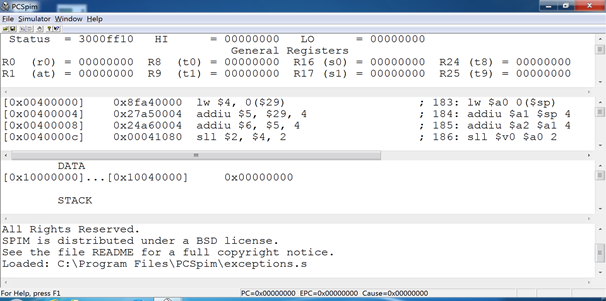
\includegraphics[width=1\linewidth]{images/fig1.png}
    \caption{The PC-SPIM user interface.}
\end{figure}

When accessed with a traditional screen reader without any additional tools, the entire content and controls of PC-SPIM can be accessed. As is visible in Figure 1, all content is textual, and thus can be presented verbally. However, the design of the user interface has not been optimized in any way to assist those using assistive technology. This results in potential significant difficulty for the student in navigating the application and accessing information being presented by the user interface. Because screen readers and speech synthesizers are generally optimized for reading English text, many aspects of the interface and code are read in a confusing or cumbersome manner. For example, the string “0(\$29)” seen in the code window above is recited as “0, left parenthesis, twenty-nine dollars, right parenthesis”. Similarly, the hexadecimal addresses are read out character by character, for example “zero x zero zero four zero zero zero zero eight”, and the assembly language mnemonics are read as if they are words; the “addiu” instruction is recited similar to the word “ado”. These are some of the shortcomings we are attempting to address with our solution.

For the screen reader, Non-Visual Desktop Access (NVDA) was chosen. Its open source nature and use of modern accessibility standards made it an excellent choice for pairing the additional Braille technologies with PC-SPIM. 

For Braille-enhanced tests, we designed a custom software interface, known to NVDA as an “add-on”, which interacts with both the IDE’s user interface and the Braille display by using the Python scripting component of the NVDA screen reader. This software provides access to various components of the IDE in real-time, allowing the software developer to quickly access information without navigating through the IDE’s numerous displays. This technique is related to the “status cells” functionality that is offered by screen readers, but in this case it is specifically designed to address the needs of a software developer using the PC-SPIM software. In addition, the custom software provides quick access to many IDE features directly from the Braille display. 

The interface provides features specific to Braille as follows:

\begin{itemize}
    \item Display the value of a variable or register in a static, non-changing area of the Braille display, allowing the user to navigate away from the content while keeping the value displayed on the Braille display.
    \item Display the value of a variable or register in real time in an area of the Braille display, allowing the user to step through a program and observe the variable’s changes over time. This is analogous to the Watch feature of modern IDEs.
    \item Parse the source code in the editor and present it in a format well suited for reading in Braille. Disorganized information is organized and presented on a line-by-line basis.
    \item Provide quick, direct navigation to the various displays of the IDE.
    \item Copy output of any display to the Clipboard. This feature is not available in the standard IDE without using the mouse and visually selecting and copying the text.
\end{itemize}

All of the above features are accessed via additional keystrokes and/or Braille commands. Each time the participant executes any of the above functions during a task, the incident is recorded. The total number of times all features are uses is recorded. Figure 2 illustrates how we display both source code and internal register information in Braille.

\begin{figure*}[!th]
    \centering
    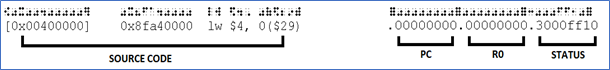
\includegraphics[width=1\linewidth]{images/fig2.png}
    \caption{An example of how Braille is used to represent source code and status indicators in the IDE. Text below the Braille cells indicates the displayed characters}
\end{figure*}

\subsection*{Hardware}

The Braille display device used for the study is the Freedom Scientific Focus 80 Blue. It has 80 display cells as well as Braille keyboard input functions. It interacts with the NVDA screen reader and the add-on we have written to provide access to the PC-SPIM software. (See Figure 3)

\begin{figure}[!h]
    \centering
    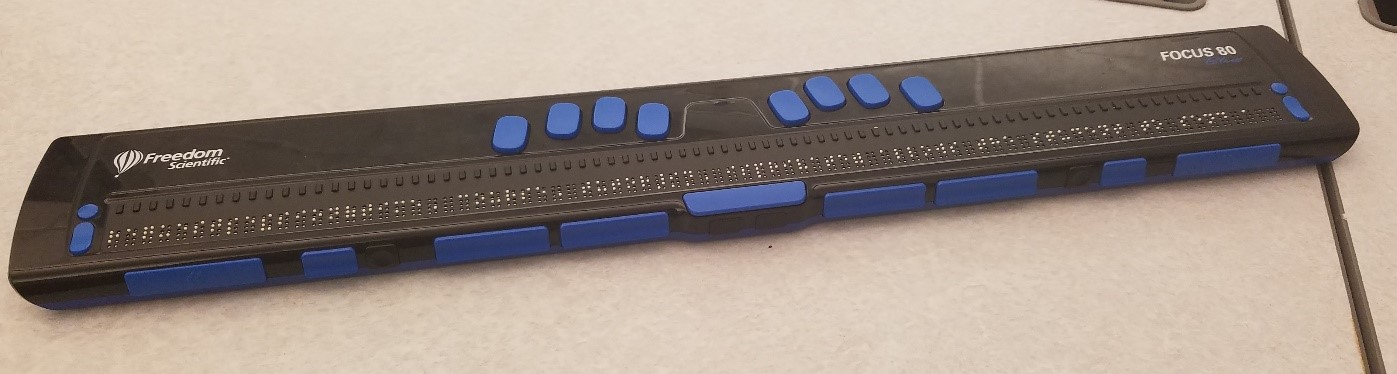
\includegraphics[width=1\linewidth]{images/fig3.jpg}
    \caption{A Freedom Scientific Focus-80 Braille display, as used in the experiment}
\end{figure}

\newpage

The screen reader and Braille device were used with an iMac desktop computer running Microsoft Windows in a virtualized environment. The keyboard used was the standard wired Apple keyboard. The mouse is not used in the experiment.

\section*{FINDINGS}

\subsection*{Time}

We have observed an average improvement in speed of 2.75x faster when the participant was using the Braille display. The average time to completion for all tasks with the use of the additional Braille hardware and software was 50.1 seconds, while the average completion without was 2 minutes and 17.8 seconds. The Kolmogorov-Smirnov normality test indicated that trials both with and without Braille had p = .2, verifying that the data is normally distributed. Thus, we performed an independent-sample T-test of use of Braille against time. Braille usage had a significant effect in favor of reduced time of completion with p < .001. Our data is illustrated in Table 1.

\begin{table}[h]
\caption{Average time taken in seconds for the participant to complete the given task.}
\begin{tabular}{ccc}
 & \textbf{Without Braille} & \textbf{With Braille} \\ \hline
Task 1 & 52.6 & .5 \\
Task 2 & 164.3 & 77.2 \\
Task 3 & 191.3 & 28.0 \\
Task 4 & 142.7 & 54.8 \\ \hline
\textbf{All Tests} & \textbf{137.8} & \textbf{50.1} \\
\end{tabular}
\end{table}

\subsection*{Braille Add-on Functionality Usage}
 
We measured the usage of the functions we provided in the Braille add-on to determine how they were used. Task 4 used the Braille functions the most of any task, and also used the most diverse set of these functions. 

\begin{table}[h]
\caption{Usage counters for Braille helper functions.}
\begin{tabular}{lcccc}
\textbf{Function} & \textbf{Task 1} & \textbf{Task 2} & \textbf{Task 3} & \textbf{Task 4} \\ \hline
Copy To Clipboard & 4 &  &  & \\
Set Focus &  &  &  & 9 \\
Show Register Values &  & 3 &  & 3 \\
Freeze Register Values &  & 3 &  & 1 \\
Parse Code &  &  & 2  & \\ \hline
\end{tabular}
\end{table}

\subsection*{User Experience}

The reported frustration level by the participant was significantly higher when not using the Braille display. On a Likert scale of 1 to 5, with 5 being the most frustrated and 1 being the least, the participant provided a response of 1 (least frustrated) for every task which included use of the Braille display. The average frustration level without Braille was 4.2. A Chi-Square test of the reported frustration level showed a significant effect of Braille in reducing the frustration level with p < .001. 

The participant found that using the Braille display made a difference in the perceived difficulty of the tasks. On a Likert scale of 1 to 4, with 1 being least difficult and 4 being most difficult, the reported average difficulty of the tasks without using the Braille display was 3.25. With Braille, the average difficulty was 1.1, with the participant reporting mild difficulty on only one task. A Chi-Square test of the reported difficulty level showed a significant effect of Braille in reducing the perceived difficulty of the tasks with p < .001.

When using Braille, the participant felt they completed the tasks in a timely manner in all cases. Without Braille, the participant felt that completion time was too long in all but one case. A Chi-Square test showed that Braille had a significant effect in favor of the perceived reasonable time to completion with p < .001.

In all cases, the participant indicated that she felt the use of Braille was beneficial and would choose to use it if it were available. These results are illustrated in Figure 4 and Figure 5.

\begin{figure}[!h]
    \centering
    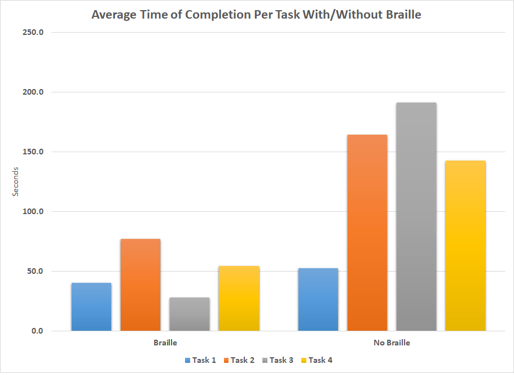
\includegraphics[width=1\linewidth]{images/fig4.png}
    \caption{Task completion times in seconds for Braille and non-Braille trials}
\end{figure}

\begin{figure}[!h]
    \centering
    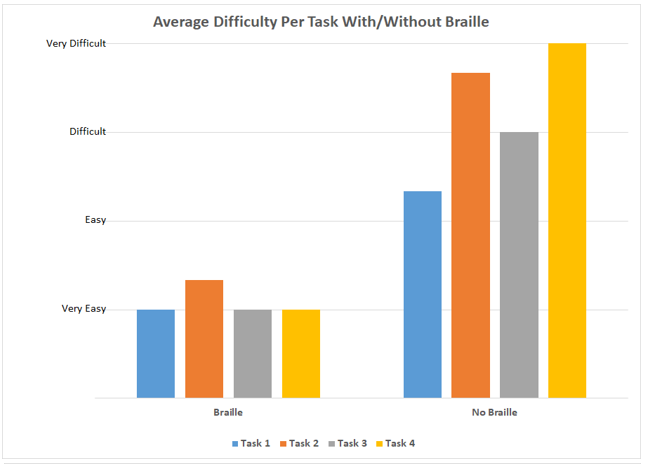
\includegraphics[width=1\linewidth]{images/fig5a.png}
\end{figure}
\begin{figure}[!h]
    \centering
     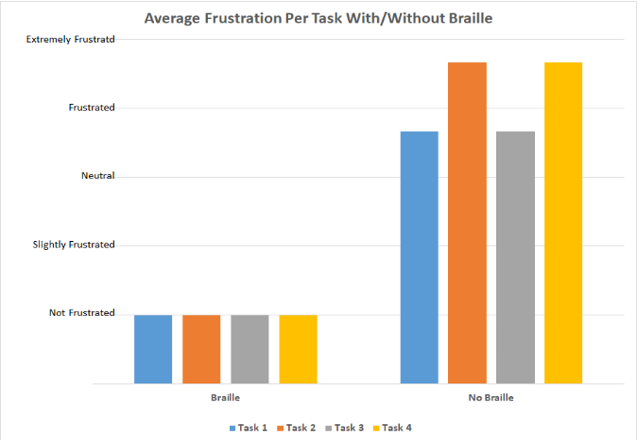
\includegraphics[width=1\linewidth]{images/fig5b.png}
    \caption{Result averages from Qualtrics survey. Lower bars mean better performance and experience.}
    
\end{figure}

\subsection*{Observations}

From the notes taken during each test, we observed that when not using the Braille display, the participant exhibited many outward signs of frustration such as the use of uncouth language and facial expressions of aggression. In many cases, the participant needed to back up and repeat parts of the task due to losing her current place in the user interface, yet another sign of undesirable user experience outcome. 

The screen reader also did not present the content to the participant in an effective way. For example, the variables were presented as a column list in a text window, but without column separation. The columns were instead presented in a monospace font with spacing used to separate them. This caused the screen reader to repeatedly read irrelevant information, thus confusing the participant when she was trying to locate the requested information.

With the additional control afforded by the Braille display, the participant was visibly more relaxed and enthusiastic about the tests. The participant quickly and easily located key pieces of information.

\subsection*{Limitations}

The PC-SPIM software is of limited practical value and is mostly used as a teaching tool for computer science courses. While adapting the PC-SPIM interface is a useful endeavor for the academic sector, this study could be expanded to account for more powerful IDEs such as Microsoft’s Visual Studio or Apple’s Xcode.

While a single-subject longitudinal study may provide generalizable results for quantifiable variables, it is not adequate for explaining the user experience of the highly diverse population of individuals with visual impairments. 

Finally, the cost of assistive technology is often prohibitive; the cost of the Focus 80 Blue product used during the study is \$7,795.00 at the time of this writing. The high cost of this equipment can limit its availability; therefore, even though this study has demonstrated significant benefits from using the Braille display, the cost may limit its application in a real-world setting. 

\section*{CONCLUSIONS}

This study serves as a demonstration of the need for more intense and detailed evaluation of the advantages that can be provided to software developers when using Braille and accompanying software to aid in information retrieval. 

The GUI is not going away, but technologies such as Braille displays and the accompanying software modules, which provide customized interfaces for them, can help give individuals who are blind the best chance of remaining competitive in the ever-evolving technology industry. 

\subsection*{Future Work}

To further the practical applications of this research, we will conduct a study with a larger number of participants to evaluate desirable and undesirable user experience outcomes from the use of software development GUIs with and without Braille. This study will utilize a mainstream IDE such as Visual Studio. 

\end{large}

\clearpage
\section*{REFERENCES}\par 
\leftskip 0.25in
\parindent -0.25in 

Alexander, S. (1998, November). Blind programmers face an uncertain future. \textit{CNN.com}. Retrieved from \url{http://www.cnn.com/TECH/computing/9811/06/blindprog.idg/}

American Printing House for the Blind. (2013). \textit{Annual report October 1, 2012-September 30, 2013}. Retrieved from \url{http://www.aph.org/files/annual-reports/APH-Annual-Report-FY13.pdf}

Chen, J., \& Takagi, N. (2014). Development of a system to assist automatic translation of hand-drawn maps into tactile graphics and its usability evaluation. \textit{Advances in Fuzzy Systems, 2014}, 1–11. doi: 10.1155/2014/357380

Edgington, E. S. (1967). Statistical inference from n = 1 experiments. \textit{The Journal of Psychology, 65}(2), 195-199. doi: 10.1080/00223980.1967.10544864

Edwards, W. K., Mynatt, E. D., \& Stockton, K. (1994). Providing access to graphical user interfaces—not graphical screens. In \textit{Proceedings of the first annual acm conference on assistive technologies} (p. 47–54). New York, NY, USA: Association for Computing Machinery. doi: 10.1145/191028.191041

Evans Data Corporation. (2014). \textit{Global developer population and demographic study vol. 2}. Retrieved from \url{https://evansdata.com/reports/viewRelease.php?reportID=9}

Freedom Scientific. (2014). \textit{Focus 40 Blue refreshable braille display user’s guide}. Retrieved from \url{https://www.freedomscientific.com/Content/Documents/Manuals/Focus/Focus40Blue/Focus-40-Blue-Online-Users-Guide.htm} 

Handy Tech. (n.d.). \textit{Company history}. Retrieved from \url{https://handytech.de/en/info/handy-tech/history}

K., M. H., \& C., S. (2014, Sep). Use of information and communication technology by visually-impaired students: A study in University of Calicut, Kerala. \textit{DESIDOC Journal of Library \& Information Technology, 34}(4), 342–348. doi: 10.14429/djlit.34.6586

Lazar, J., Allen, A., Kleinman, J., \& Malarkey, C. (2007). What frustrates screen reader users on the web: A study of 100 blind users. \textit{International Journal of Human–Computer Interaction, 2}2(3), 247-269. doi: 10.1080/10447310709336964 

Mealin, S., \& Murphy-Hill, E. (2012). An exploratory study of blind software developers. In \textit{2012 IEEE symposium on visual languages and human-centric computing (VL/HCC)} (p. 71-74).

Microsoft Corporation. (2018, May). \textit{Microsoft active accessibility technical overview}. Retrieved from \url{https://msdn.microsoft.com/en-us/library/dd373660.aspx}

Mynatt, E. D., \& Weber, G. (1994). Nonvisual presentation of graphical user interfaces: Contrasting two approaches. In \textit{Conference companion on human factors in computing system}s (p. 211). New York, NY, USA: Association for Computing Machinery. doi: 10.1145/259963.260338

National Federation of the Blind. (2014). \textit{Blindness statistics: Statistical facts about blindness in the United States}. National Federation of the Blind. Retrieved from \url{https://nfb.org/blindness-statistics}

Onghena, P. (1992). Randomization tests for extensions and variations of abab single-case experimental designs: A rejoinder. \textit{Behavioral Assessment, 14}(2), 153-171.

Stack Overflow. (2017). \textit{Developer survey results 2017}. Retrieved from \url{https://insights.stackoverflow.com/survey/2017}

Takagi, H., Saito, S., Fukuda, K., \& Asakawa, C. (2007, September). Analysis of navigability of web applications for improving blind usability. \textit{ACM Trans. Comput.-Hum. Interact., 14}(3), 13–es. doi: 10.1145/1279700.12\\79703

Van Gerven, C., \& Taylor, A. (2009). The information age braille technology timeline. \textit{Future Reflections, 28}(1). Retrieved from \url{https://www.nfb.org/sites/} \url{www.nfb.org/files/images/nfb/publications/fr/fr28/fr280109.htm}

WebAIM. (2013). \textit{Visual disabilities: How blind people use the web}. Author. Retrieved from \url{https://webaim.org/articles/visual/blind}

WebAIM. (2015). \textit{Screen reader user survey \#6 results}. Author. Retrieved from \url{https://webaim.org/articles/visual/blind}

Wobbrock, J. O., Kane, S. K., Gajos, K. Z., Harada, S., \& Froehlich, J. (2011, April). Ability-based design: Concept, principles and examples. \textit{ACM Trans. Access. Comput., 3}(3). doi: 10.1145/1952383.1952384

\clearpage
\begin{large}

\leftskip 0in
\parindent 0in 

\section*{APPENDIX} 
The source code used in this experiment is available at the following repository: \url{https://www.github.com/fmillion/pcspim-nvda}

The source code for this project is licensed under the GNU General Public License (GPLv3). Source code has been updated to function with the current version of NVDA, which is 2019.1 at the time of this writing. 

\end{large}
\end{document}